%%%%%%%%%%%%%%%%%%%%%%%%%%%%%%%%%%%%%%%%%%%%%%%%%%%%%%%%%%%%%%%%%%%%%%%%%%
%% 卒論中間・卒論前刷・修論中間、全部同じなのに、
%% ファイルが3つあったので、共通の部分を取り出した。by 水内(2020年春)
%%%%%%%%%%%%%%%%%%%%%%%%%%%%%%%%%%%%%%%%%%%%%%%%%%%%%%%%%%%%%%%%%%%%%%%%%%
% 東京農工大学 工学部 機械システム工学科 卒論発表前刷り用スタイルファイル
% Thanks to 佐久間先生 and 佐久間研の皆さん
% 書式設定部分のみ分離&いくつかコマンド定義&微修正 by 本堂
% 中間発表前刷り用スタイルを卒論発表用に改造 by 本堂
% 2013年度版でテンプレートに変更点があったので修正 by 恒岡
% 2016年度版でテンプレートに変更点があったので修正 by 熊谷
%%%%%%%%%%%%%%%%%%%%%%%%%%%%%%%%%%%%%%%%%%%%%%%%%%%%%%%%%%%%%%%%%%%%%%%%%%

\documentclass[a4paper,twocolumn,twoside,fleqn,leqno,10pt,dvipdfmx]{jarticle}


\usepackage[dvipdfmx]{graphicx}
\usepackage[dvipdfmx]{color}
\usepackage{bm}
\usepackage{fancyhdr}
%\usepackage{nidanfloat}
\usepackage{float}
\usepackage{booktabs}
\usepackage{amsmath}
\usepackage{amssymb}

\usepackage[dvipdfmx]{hyperref}  % 目次や参考文献をリンクにする。
\hypersetup{bookmarksnumbered=true}
\hypersetup{colorlinks=true}
\hypersetup{linkcolor=black}
\hypersetup{citecolor=black}

\usepackage{url} % \url のために必要。パッケージが無い人は探して入れる。
%% \url{http://nile.ulis.ac.jp/~yuka/}のようにして使う。

\hypersetup{urlbordercolor={1 1 1}} %(ここから)URLがマゼンダで表示されちゃうのを黒に直す
\hypersetup{bookmarksnumbered=true}
\hypersetup{linkcolor={0 0 0}}
\hypersetup{linkbordercolor={1 1 1}}
\hypersetup{colorlinks=false}
\hypersetup{citebordercolor={1 1 1}}%URLがマゼンダで表示されちゃうのを
                                %黒に直す(ここまで)

%微分演算子関係
\newcommand{\dd}{\mathrm{d}} %微分演算子の"d"はローマン体
\newcommand{\diff}[2]{\frac{\mathrm{d}#1}{\mathrm{d}#2}} %常微分
\newcommand{\ddiff}[3]{\frac{\mathrm{d}^#1 #2}{\mathrm{d} #3^#1}} %高階常微分
\newcommand{\pdiff}[2]{\frac{\partial #1}{\partial #2}} %偏微分
\newcommand{\pddiff}[3]{\frac{\partial^#1 #2}{\partial #3^#1}} %高階偏微分

% 以下書式設定(一般) %%%%%%%%%%%%%%%%%%%%%%%%%%%%%%%%%%%%
\setlength{\hoffset}{-5mm}
\setlength{\voffset}{-9mm}
\setlength{\oddsidemargin}{0mm}
\setlength{\evensidemargin}{\oddsidemargin}
\setlength{\topmargin}{0mm}
\setlength{\headheight}{0mm}
\setlength{\headsep}{0mm}
\setlength{\textwidth}{180mm}
\setlength{\textheight}{255mm}
\setlength{\columnsep}{10mm}
\setlength{\topskip}{19.00pt}
\setlength{\mathindent}{4mm}
%\setlength{\kanjiskip}{0.00zw plus.1zw}
\setlength{\kanjiskip}{0.05zw plus.1zw}

\setlength{\floatsep}{3pt plus 1pt minus 1pt}
\setlength{\textfloatsep}{5pt plus 1pt minus 0.5pt}
\setlength{\intextsep}{5pt plus 1pt minus 0.5pt}
\setlength{\dblfloatsep}{3pt plus 1pt minus 1pt}
\setlength{\dbltextfloatsep}{3pt plus 1pt minus 1pt}

\setlength{\parskip}{0pt}
\setlength{\parindent}{1zw}
\setlength{\partopsep}{0pt}

% 英文概要設定 %
\def\abstract{\list{}{\listparindent=1zw \itemindent=\listparindent%
\leftmargin=5mm \rightmargin=\leftmargin}\item[]
\let\endabstract\endlist}

% 脚注の設定 %
\def\thefootnote{}

% 各節タイトル %
\def\thesection {\arabic{section}.}
\def\thesubsection {\arabic{section}$\,\cdot\,$\arabic{subsection}}
\def\thesubsubsection {\thesubsection$\,\cdot\,$\arabic{subsubsection}}

% 数式環境 %
\newdimen\vs % 機械学会書式(added by A.Sakuma)
\def\gyo[#1]{\\ \vbox to#1\vs\bgroup\vss}
\def\endgyo{\vss\egroup\vspace{-1.2mm}}%
\def\LABEL#1{\dotfill\hspace*{9.0mm}\label{#1}}
\def\LABELW#1{\dotfill\hspace*{23.0mm}\label{#1}}
\def\DOTFILL#1{\unitlength=1mm\begin{picture}(#1,3)
 \put(0,0){\makebox(#1,1.5)[b]{\dotfill}}\end{picture}}

% 図の配置設定 %
\def\topfraction{1.0} % 機械学会書式(changed by A.Sakuma)
\setcounter{bottomnumber}{6} % 機械学会書式(changed by A.Sakuma)
\def\bottomfraction{1.0} % 機械学会書式(changed by A.Sakuma)
\setcounter{totalnumber}{8} % 機械学会書式(changed by A.Sakuma)
\def\textfraction{0.0} % 機械学会書式(changed by A.Sakuma)
\def\floatpagefraction{0.7} % 機械学会書式(changed by A.Sakuma)
\setcounter{dbltopnumber}{8}% 機械学会書式(changed by A.Sakuma)
\def\dbltopfraction{1.0} % 機械学会書式(changed by A.Sakuma)
\def\dblfloatpagefraction{0.7} % 機械学会書式(changed by A.Sakuma)
% ```````````````````````````````````````````````````````
% 以下書式設定(特殊) %%%%%%%%%%%%%%%%%%%%%%%%%%%%%%%%%%%%
\makeatletter

% 各節タイトル %
\def\section{\@startsection {section}{1}{0.0ex}{1.62ex}{1.62ex}{\center\bf}}%%セクションを太字に2018諸岡
\def\subsection{\@startsection{subsection}{2}{0.0ex}{1.0ex}{.5ex}{\rm}}%タイトルの後改行
%タイトルを中央揃えにする場合は@startsectionの第6引数を{\center\bf}にする
\def\subsubsection{\@startsection{subsubsection}{3}{3.0ex}{0.0ex}{-6.0ex}{\rm}}

\def\quote{\list{}{\rightmargin=10mm \leftmargin=\rightmargin}\item[]}%
\long\def\@makecaption#1#2{
\vskip 10pt 
\setbox\@tempboxa\hbox{#1  #2}
\ifdim \wd\@tempboxa >\hsize \settowidth{\labelwidth}{#1} \textwidth=\hsize
\addtolength{\textwidth}{-\labelwidth}\addtolength{\textwidth}{-6pt}
\tabcolsep=2pt\begin{tabular*}{\hsize}{@{\extracolsep{\fill}}lp{\textwidth}}
 #1&\setlength{\baselineskip}{9.0pt}\setlength{\lineskip}{-0.5pt}#2\\
 \end{tabular*}\par\else\hbox to\hsize{\hfil\box\@tempboxa\hfil} \fi}

\def\fnum@figure{\small{Fig.\thefigure}}

% 引用の設定 %
\def\@cite#1#2{$^{\hbox{\scriptsize({#1\if@tempswa , #2\fi})}}$}
\def\thebibliography#1{\section*{{\bf 文  献}\@mkboth
 {REFERENCES}{REFERENCES}}\list
% {(\hfill\arabic{enumi}\hfill)}{\settowidth\labelwidth{1pt} \leftmargin 30pt
 {(\hfill\arabic{enumi}\hfill)}{\settowidth\labelwidth{1pt} \leftmargin\labelwidth %文献のインデントを左端にした。
 \advance\leftmargin\labelsep
 \usecounter{enumi}}
 \def\newblock{\hskip .11em plus .33em minus .07em}
 \sloppy\clubpenalty4000\widowpenalty4000
 \sfcode`\.=1000\relax}

% 数式環境 %
\def\@eqnnum{\hbox to .01pt{}
 \rlap{\rm \hskip -0.125\displaywidth(\theequation)}}
\def\eqnarray{\stepcounter{equation}\def\@currentlabel{\p@equation\theequation}%
 \global\@eqnswtrue\m@th\global\@eqcnt\z@\tabskip\@centering\let\\\@eqncr
 $$\everycr{}\halign to\displaywidth\bgroup\hskip\@centering$\displaystyle
 \tabskip\z@skip{##}$\@eqnsel&\global\@eqcnt\@ne \hfil$\displaystyle{{}##{}}$\hfil
 &\global\@eqcnt\tw@ $\displaystyle{##}$\hfil\tabskip\@centering
 &\global\@eqcnt\thr@@ \hb@xt@\z@\bgroup\hss##\egroup\tabskip\z@skip\cr}  
\def\@eqnnum{\hbox to .01pt{}%
 \rlap{\rm \hskip -0.10\displaywidth(\theequation)}}
\def\fnum@table{Table \thetable.}
\def\thetable{\@arabic\c@table}

%% Figure 環境中で Table 環境の見出しを表示・カウンタの操作に必
\newcommand{\figcaption}[1]{\def\@captype{figure}\caption{#1}}
\newcommand{\tblcaption}[1]{\def\@captype{table}\caption{#1}}

\makeatother

\usepackage{ifthen}
\newcommand{\secret}[2]{
  \ifthenelse{\equal{#1}{m}}{
    \thispagestyle{fancy}
    \lhead{
      \vspace{-10mm}
      \begin{picture}(0,0)
        \fboxrule=0.5mm
        \hspace{#2}\fcolorbox{red}{white}{{\large {\bf \textcolor{red}{専攻外秘}}}}
    \end{picture}
    }
  }{
    \thispagestyle{fancy}
    \lhead{
      \vspace{-10mm}
      \begin{picture}(0,0)
        \fboxrule=0.5mm
        \hspace{#2}\fcolorbox{red}{white}{{\large {\bf \textcolor{red}{学科外秘}}}}
      \end{picture}
    }
  }
}

\newcommand{\pagenum}[1]{%
\chead{}
\rhead{ \sf{#1} }%%フォントを変更2018諸岡
\lfoot{}
% \cfoot{ \bf{#1} } %ページ数
\cfoot{}
\rfoot{}
}

\renewcommand{\headrulewidth}{0pt}
\renewcommand{\footrulewidth}{0pt}

\newcommand{\smallcap}[1]{\vspace{-1pt}\caption{{\footnotesize #1}}}

\pagestyle{empty}
\renewcommand{\title}[2]{
%\twocolumn[%
 \begin{center}
 {\Large\bf #1}\\%日本語タイトルも太字に変更2018諸岡
 {\bf #2}%英語タイトル太字に変更
\end{center}
\vspace{-5mm}
}

\renewcommand{\author}[3]{
 \begin{flushright}
  \begin{small}
    #1\hspace{6mm}#2\hspace{3mm}#3\\
%% #1  #2 
%% #3   \\
  \end{small}
 \end{flushright}
}



% キーワード
\newcommand{\keyword}[1]{
 \begin{center}{\small
  \begin{tabular*}{150mm}{lp{140mm}}
    \hspace{-17mm}\sl{Key Words} %%Key Word(細字イタリック)に変更2018諸岡
    \rm{: #1}
  \end{tabular*}
 }\end{center}
\vspace{-3mm}
}

\usepackage{setspace}
\renewenvironment{abstract}{\begin{small}\begin{spacing}{1}\hspace{6mm}}{\end{spacing}\end{small}\vspace{-3mm}}

\setlength{\vs}{\baselineskip}
\vspace{-\baselineskip}
\setlength{\baselineskip}{4.30mm}


\pagenum{\bf B-208}%ページ番号 プログラムが確定したら修正を!
\secret{b}{0mm}                 %学外秘/専攻外秘の設定.学部はb(学外秘),修士はm(専攻外秘)にする.
                                %第2引数は位置の調整用.-側に大きくすれば左に寄る.+側に大きくすれば右に寄る.

\newcommand{\FIGDIR}{./fig}	%図を置くディレクトリを指定する
				%Makefileとは連動していないので注意
\usepackage{pxjahyper} %% これを入れるとしおりが文字化けしない.out2uniが不要になる.
\usepackage{ikuo}%%便利コマンド集.
\hypersetup{
  pdfborder={0 0 0}   % リンクの枠線を無効化
}


\begin{document}
\twocolumn[%
\title{伸縮する単リンクブラキエーションロボットの

ロバストな自在移動の実現}{Realization of robust movement to arbitrary locations by an extensible single-rod brachiation robot}
\author{水内研究室}{大澤 蒼人}{Aoto OSAWA}
]
\begin{small}
\vspace{-2mm}
\section{緒  言}
\vspace{-2.5mm}
ブラキエーションは,上肢で枝を掴んでぶら下がりながら移動する方法であり,
重力を利用することで高所を効率的に移動できる.
これをロボットに応用することで\cite{福田敏男1990ブラキエーション形移動ロボットの研究},送電線の点検などの高所作業への応用が期待されている.
従来のブラキエーションロボットはテナガザルを模倣した多リンク型であった.
しかし,多リンク型はカオス現象のような非周期的な運動が発生するため
制御が難しいという問題がある\cite{鈴木三男2000二重振り子におけるカオス的振舞}.
先行研究では,単リンク,すなわち棒状にすることにより問題を解決した.
さらに振子過程で,リンクが伸縮する機構を用いてブランコを漕ぐように
振動を拡大させ(これを励振と呼ぶ),適切なタイミングでリンクを伸ばすことで,
ロボットの最大長と等しい距離にある同じ高さのバーへの移動を実機で実現した\cite{Hijiri:Robomech2024}.
しかし,この移動は常にグリッパーがバーを把持しており,移動可能距離はロボットの最大長までである.
また,2次元方向移動のみに限定されている.
そのため,バーを離して飛び移る「空中過程」を含む移動や,3次元方向移動,
さらには揺らぎやバーを離す際の不確実性・外乱に応じた動作再計画の実現までには至っていない.
そこで,本研究では伸縮する棒状ブラキエーションロボットの自在移動を実現させるとともに,
ロバスト性を高めることを目的とする.
\vspace{-2.65mm}
\section{実現手法}
\vspace{-2.5mm}
本研究では,次のバーまでの距離から
現在把持しているバーを離す条件(バーリリース条件)を導くことで,
最適な移動を行う.さらに,3次元方向移動を可能にする機構を構築することで
自在な移動を実現する.また,再計画により安定した移動を実現させる.
以下に実現手法を示す.
\vspace{-1mm}
\subsection{バーの認識と最適なバーリリース条件の導出}
\subseclabel{バーリリースタイミング}
\vspace{-1mm}
ロボットとバーの模式図を\figref{figone}に示す.
グリッパーの側面に測距センサを取り付け,次のバーの距離を測定し,
グリッパーと次のバーとの距離に基づいた\equref{J}に示す評価関数$J$を考える.
ここで,$(l_{\mathrm{bx}},l_{\mathrm{bz}})$は次のバーの座標を示し,
$(x_{\mathrm{e}},z_{\mathrm{e}})$はグリッパーの手先座標を表す.
手先座標は\equref{x-z}に示すように,重心座標$(x_{\mathrm{c}},z_{\mathrm{c}})$,バーリリース時のロボットの長さ$l_{\mathrm{r}}$,角度$\varphi$,角速度$\dot{\varphi}$とバーリリース後の時刻$t$から求まる.
なお,空中過程におけるロボットの長さはバーリリース時の長さのままであるとして求める.
% \vspace{-1mm}
\setlength{\abovedisplayskip}{2pt}
\setlength{\belowdisplayskip}{3pt}
\begin{eqnarray}
    \equlabel{J}
    J(\varphi,\dot{\varphi},&t,l_{\mathrm{r}})
    =\sqrt{(l_{\mathrm{bx}}-x_{\mathrm{e}})^2+(l_{\mathrm{bz}}-z_{\mathrm{e}})^2}
    \equlabel{J}
    \end{eqnarray}
% \begin{eqnarray}
%     \equlabel{x-z}
%     x_{\mathrm{e}}=x_{\mathrm{e}}(\varphi,\dot{\varphi},t,l_{\mathrm{r}}),\quad z_{\mathrm{e}}=z_{\mathrm{e}}(\varphi,\dot{\varphi},t,l_{\mathrm{r}})
%     \end{eqnarray}   
% \vspace{-1mm} 
\begin{eqnarray}
        \equlabel{x-z}
        \begin{split}
        x_{\mathrm{e}}=x_{\mathrm{c}}(t)+l_{\mathrm{r}}\sin(\varphi+\dot{\varphi}t)/2\\
        z_{\mathrm{e}}=z_{\mathrm{c}}(t)-l_{\mathrm{r}}\cos(\varphi+\dot{\varphi}t)/2
        \end{split}
        \end{eqnarray}
        % \vspace{-1mm} 
各角度・角速度において評価関数の最小値と,最小にする時刻が決まる.
この時刻におけるバー把持時のバーに対するグリッパーの相対速度と
評価関数がともに小さくなる角度・角速度の組を
最適なバーリリース条件とする.
\vspace{-1mm}
\subsection{3次元方向移動機構}
\vspace{-1mm}
グリッパーと伸縮機構の間にモーターを取り付け,
グリッパー回転が可能な機構を考える.
これによりバーに応じた方向転換が可能になるが,
現在のロボットの構造上,励振には初期振幅が必要である.
そのため,初期振幅を生成する機構・方向転換のタイミングの検討を行う.
\vspace{-1mm}
\subsection{励振計画}
\vspace{-1mm}
\subsecref{バーリリースタイミング}にて求めた最適なバーリリース条件を基に,
力学的エネルギーと外力による減衰量から目標振幅を求める.
目標振幅を実現するために,
励振過程における振幅増加量・減少量から励振計画を決定する.
なお,ロボットの角度・角速度は慣性計測ユニット(IMU)を用いて計測し,
最適なバーリリース条件を満たした時にバーを離し,空中過程へと移る.
条件を満たさない場合は目標振幅を調整し,励振再計画を行う.
また,Lieskovsk{\`y}らの研究\cite{lieskovsky2023optimal}
を基に,IMUによるフィードバック制御でリンクを伸縮させて励振する.
\subsection{空中過程における動作再計画}
\vspace{-1mm}
最適なバーリリース条件を決定した場合でも,バーリリース時のバーとの接触などの外乱により
計画していた手先軌道からずれる可能性がある.
そこで,計画と実際の手先軌道の誤差を基にフィードバック制御により
ロボットの長さ変更動作の再計画を行い,手先軌道を修正する.
手先軌道の誤差は,IMUを用いて空中過程におけるロボットの姿勢を一定時間ごとに計測することにより求める.
\vspace{-2.5mm}
\section{最適なバーリリース条件の導出とリリース実験}
\vspace{-2mm}
目標とするバー座標を(0.79m,0m),ロボットの長さを0.74mとし,
\subsecref{バーリリースタイミング}で示した評価関数$J$を導出した.
バー把持可能距離を5mmとし,導出した評価関数の最小値のうち,5mm未満となった角度・角速度のプロットを\figref{fig:two}に示す.
評価関数と,バーに対するグリッパーの相対速度がともに小さくなる組は
(67deg, 200deg/s)であった.
この角度・角速度でバーリリースを行い,バー把持に成功した.
% これによりバー座標(0.79m,0m)における最適なバーリリース条件が求まった.
\begin{figure}[t]
    \begin{center}
    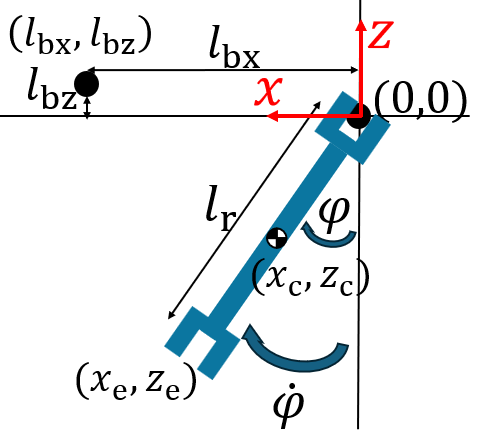
\includegraphics[width=38mm,height=32mm]{./fig/bar-robot6.png}
    \vspace{-5mm}
    \caption{Schematic Diagram}
    \vspace{-3mm}
    \figlabel{figone}
    \end{center}
    \end{figure}
\begin{figure}[t]
    \begin{center}
    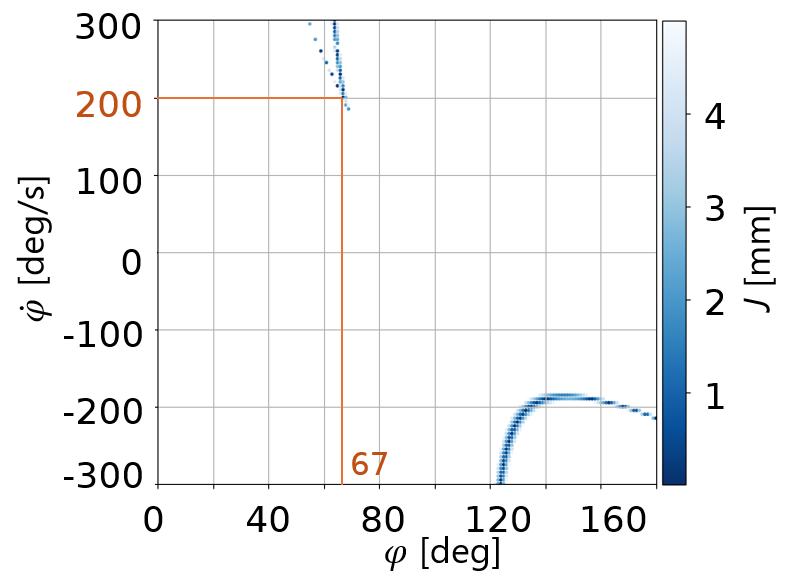
\includegraphics[width=55mm,height=40mm]{./fig/2Dver6_4.png}
    \vspace{-6mm}
    \caption{Scatter Plot}
    \vspace{-7.5mm}
    \figlabel{fig:two}
    \end{center}
    \end{figure}
\vspace{-2.8mm}
\section{結  言}
\vspace{-2mm}
本稿では,伸縮する単リンクブラキエーションロボットの
自在移動を可能にする機構と動作計画手法,
そして空中過程における動作再計画手法を提案した.
また,次のバーの座標に基づいた最適なバーリリース条件の導出を行い,実機実験によりバー把持が可能であることを確認した.
今後は,自在移動のための機構構築と,
最適なバーリリース条件実現のための励振計画・再計画プログラムを作成する.
さらに,空中過程での動作再計画によりロバスト性を高める.
\vspace{-5mm}
{
% \small
%  \setlength{\kanjiskip}{0.0zw plus.01zw} %
%  \setlength{\baselineskip}{9pt}        %
%  \setlength{\itemsep}{0.2pt}             %
%  \setlength{\lineskip}{0pt}              %
\scriptsize %%←どうしても入らない時は,このコメントをはずすと少し小さくなる.
% \vspace{-2.5mm}
\bibliographystyle{junsrt}
% \bibliographystyle{jabbrv}
\bibliography{reference}

}



%% \end{thebibliography}
\end{small}
\end{document}


% \begin{figure}[t]
%     \begin{minipage}{0.46\hsize}
%      \begin{center}

%         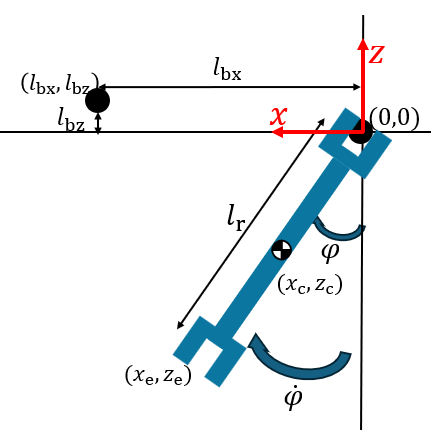
\includegraphics[width=40mm]{./fig/bar-robot5.png}
     
%     \end{center}
%     \vspace{-3mm}
%      \caption{Schematic Diagram}
%      \vspace{-3mm}
%      \figlabel{figone}
%     \end{minipage}
%     \begin{minipage}{0.50\hsize}
%      \begin{center}
      
%         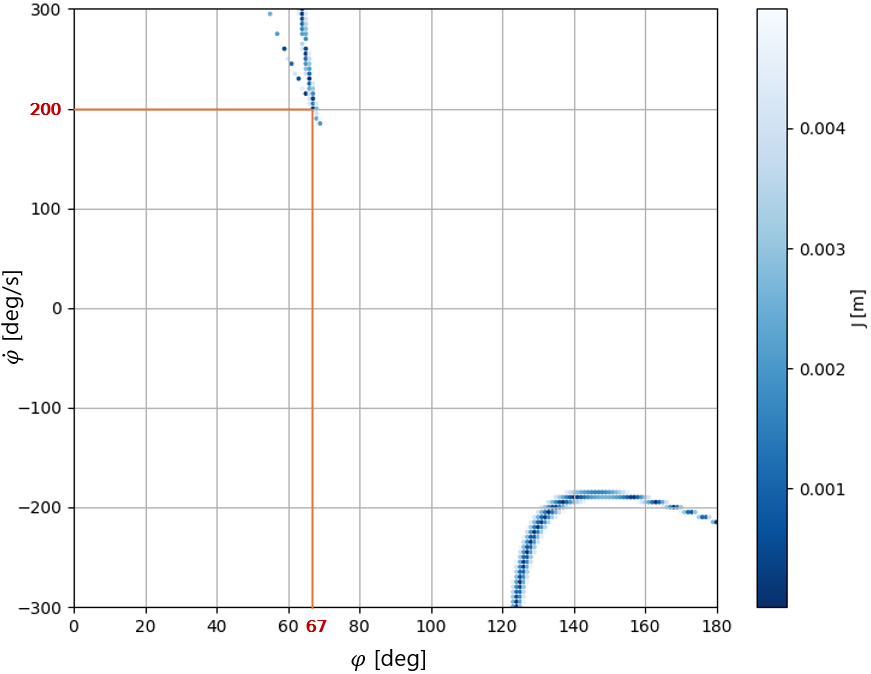
\includegraphics[width=52mm]{./fig/2Dver6_2.png}
     
%     \end{center}
%     \vspace{-3mm}
%      \caption{Scatter Plot}
%      \vspace{-3mm}
%      \figlabel{fig:two}
%     %  \vspace{5mm}
%     \end{minipage}
%    \end{figure}

% \begin{figure}[t]
%     \begin{minipage}{0.43\hsize}
%      \begin{center}

%         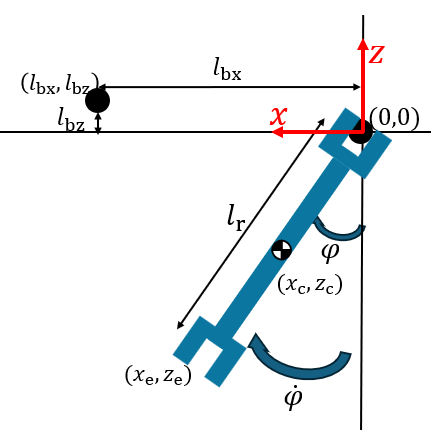
\includegraphics[width=38mm]{./fig/bar-robot5.png}
     
%     \end{center}
%     \vspace{-2.5mm}
%      \caption{Schematic Diagram}
%      \vspace{-3mm}
%      \figlabel{figone}
%     \end{minipage}
%     \begin{minipage}{0.50\hsize}
%      \begin{center}
      
%         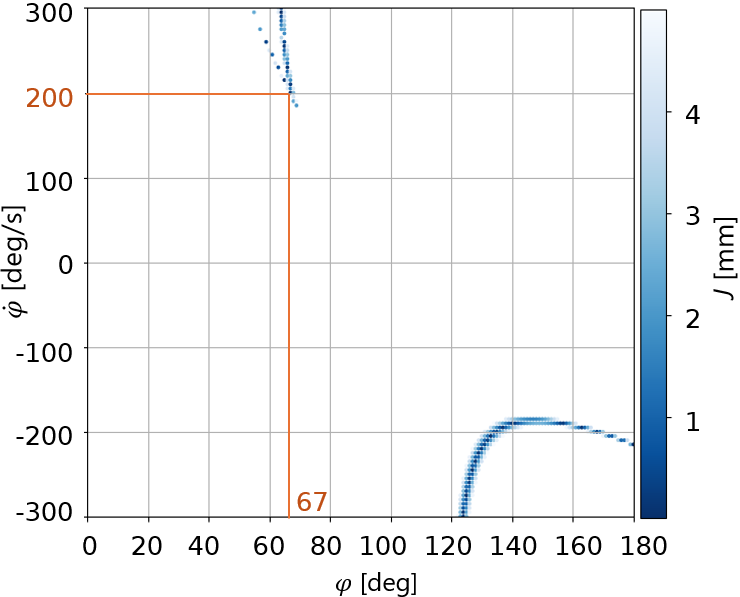
\includegraphics[width=53mm]{./fig/2Dver6_3.png}
     
%     \end{center}
%     \vspace{-7mm}
%      \caption{Scatter Plot}
%      \vspace{-3mm}
%      \figlabel{fig:two}
%     \end{minipage}
%    \end{figure}

%    \fig{bar-robot5.png}{width=.3\hsize}{The concept of hoge}
%    \fig{2Dver6_2.png}{width=.7\hsize}{The concept of hoge}
